\section{Benchmark Datasets and Workload}
We briefly discuss how we designed the benchmark datasets and corresponding workload.

\subsection{Datasets}
From publically available sources, we constructed datasets to simulated many envisioned use cases of \textsf{DeepLens}. An important consideration was images of varying format and size. Most academic benchmarks in the machine learning community consist of ``natural images'' in the same format and resolution. We decided that it was important to evaluate a diversity of tasks and the robustness of the injestion pipeline to different formats, sizes, and content. 

\vspace{0.25em} \noindent \textbf{PC.} This dataset is designed to simulate a dataset of images found on a personal computer. It consists of 779 consisting of photographs, screenshots, and document scans. 

\vspace{0.25em} \noindent \textbf{TrafficCam.} This dataset consists of 24 mins and 30 secs of high-definition (1080p) traffic camera video. 

\vspace{0.25em} \noindent \textbf{Football.} This dataset consists of 15 low-definition (720p) videos of American football clips of the same team ranging from 30 secs to 1 mins. 

\subsection{Queries}
We propose a benchmark workload of 6 queries on these datasets to evaluate \textsf{DeepLens}. These queries are inspired by problems considered in prior work and consist of task that involve querying pixel data, the results of neural network predictions, relating results back to base data, and combinations.

\vspace{0.25em} \noindent \textbf{q1.} \emph{Find all near-duplicates in the PC dataset}. This query is inspired by classical multimedia information retrieval problems such as reverse image search (find the closest image to a query image). 

\vspace{0.25em} \noindent \textbf{q2.} \emph{Count all of the frames with at least one vehicle present in the TrafficCam dataset}. This query is inspired by recent work that uses neural networks to analyze traffic and movement patterns~\cite{kang2017noscope}. This is a simple query that takes the output of a neural network that identifies objects in the frame and simply queries the output.

\vspace{0.25em} \noindent \textbf{q3.} \emph{Track one player's trajectory in every play in the Football dataset}. Given segmentation output that identifies a player in frame and OCR output that identifies a number if one is visible, we have to relate that sequence of bounding boxes back to the original image.

\vspace{0.25em} \noindent \textbf{q4.} \emph{Count all distinct pedestrians in the TrafficCam dataset}. This query is a variant of q2. The distinct qualifier makes this query significantly more challenging as it requires deduplicating candidate pedestrians detected in the video.

\vspace{0.25em} \noindent \textbf{q5.} \emph{Lookup the presence of a string in the PC dataset}. Apply OCR to all of the images, and store a collection of strings discovered. We run a query to identify the first image with a target string.

\vspace{0.25em} \noindent \textbf{q6.} \emph{Find all tuples of pedestrians (p1,p2) where p1 is behind p2 in the TrafficCam dataset}. This query is inspired from applications in robotics and navigation, where one has to estimate how far a given object is located from a camera. This problem, called depth prediction, has recently been a subject of research interest in computer vision~\cite{depthPredictModel}. We leverage the published code~\footnote{https://github.com/iro-cp/FCRN-DepthPrediction} and the pre-trained parameters to annotate all detected pedestrians in the TrafficCam dataset with depth predictions and find such pairs.

\section{Experiments}
\textbf{TODO: below all needs to be revised}
We present results on the benchmark dataset and queries to illustrate some of the key open research challenges in the design of such systems.
Our baseline is the dataflow query processing engine with no indexes.
We compare this baseline to a hand-tuned version where we manually select the best physical design for a query.

\begin{figure}[t]
% \vspace{-5pt}
\centering
 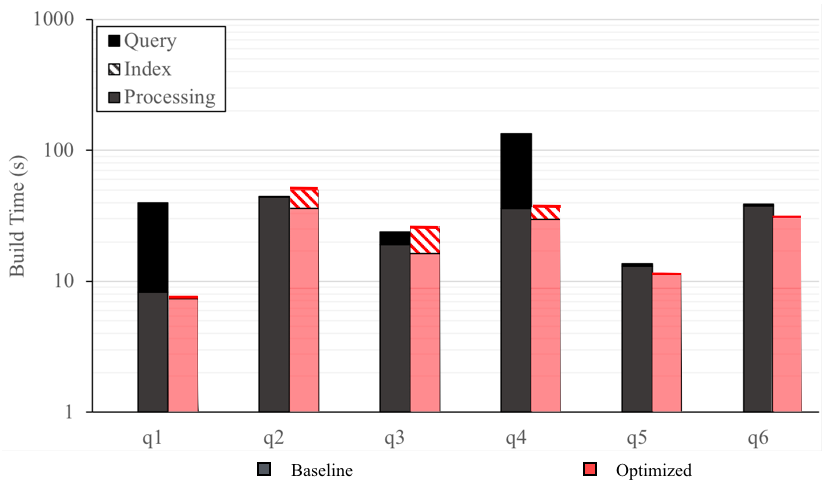
\includegraphics[width=\columnwidth]{figures/indexing1.png}
 \caption{On-the-fly index creation is beneficial. We evaluate the pipeline runtime, including ETL and index creation, for an optimized \textsf{DeepLens} (red) vs. the baseline (black). On many queries it is beneficial to materialize intermediate results and build indexes to speed up future performance. \red{The legend is unclear - Query and processing have almost the same background color - we should change it to more distinctive ones, e.g. blue and green with some patterns.} \label{index} }
\end{figure}

\begin{figure}[t]
% \vspace{-5pt}
\centering
 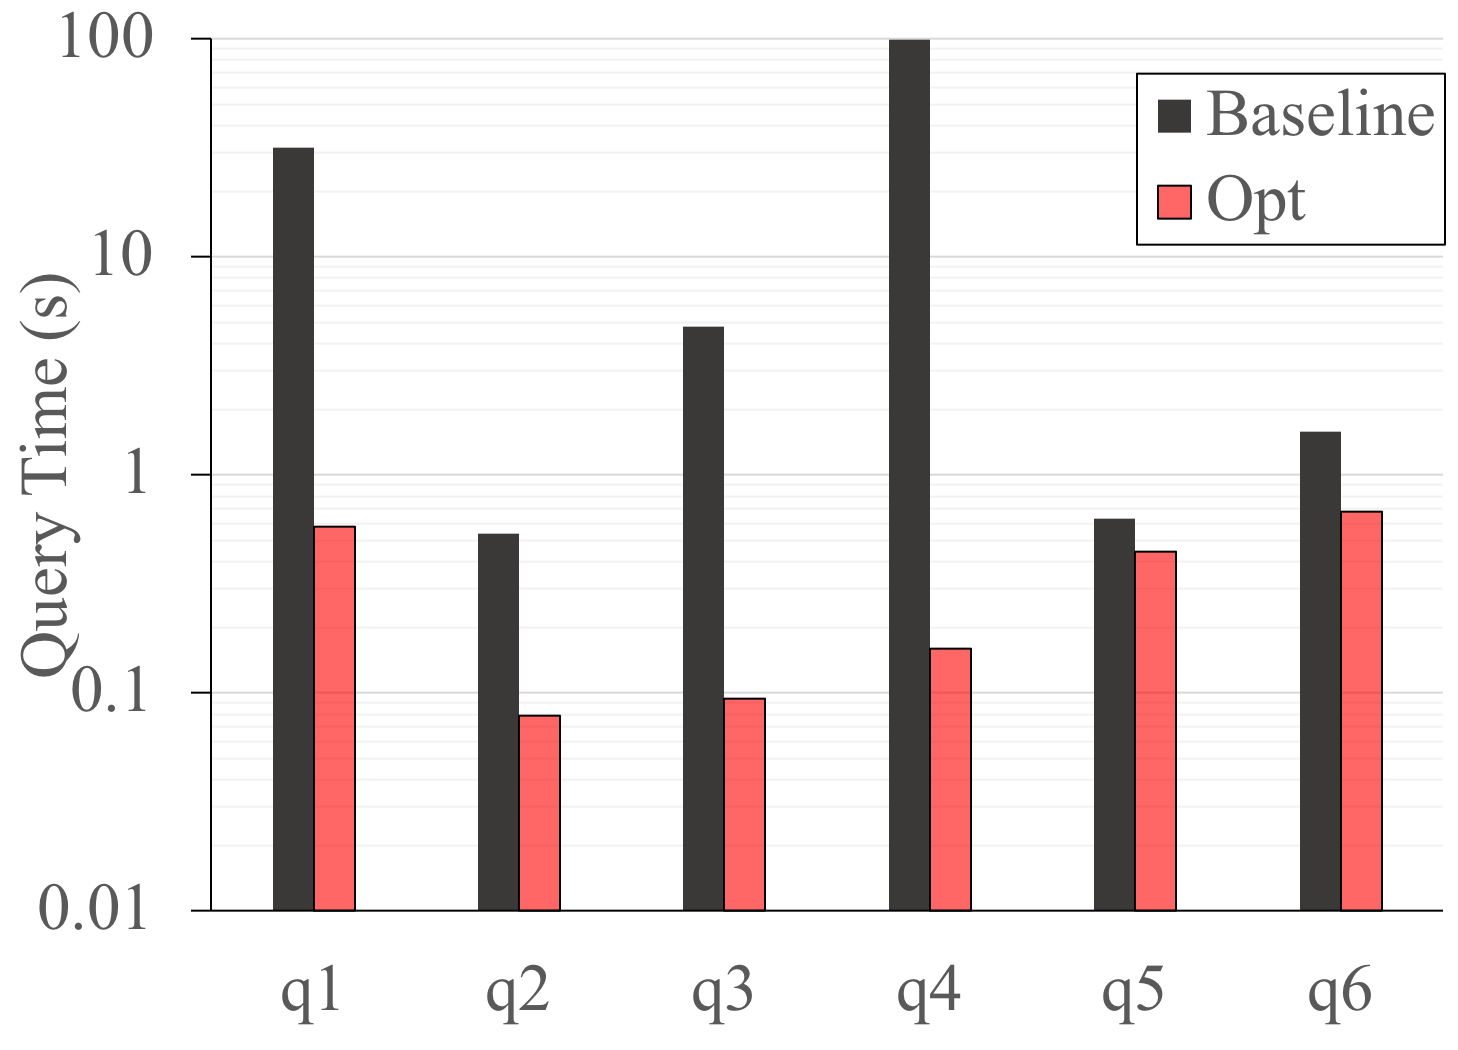
\includegraphics[width=\columnwidth]{figures/query.png}
 \caption{\textsf{DeepLens} significantly speeds up ``query time'' after building the indexes off-line.  \label{query} }
\end{figure}

\subsection{On-the-fly Indexing}
In most RDBMS, we usually consider index creation as an offline task that can amortize its benefits over an entire workload.
One surpsrising result is that for many visual analytics queries, on-the-fly index creation is beneficial (Figure \ref{index}), where materializing and indexing intermediate results reduces the execution time of future stages.
For example, q1 executes nearly 5 times faster than the baseline and q4 executes 3.5 times faster than the baseline.
If we consider only the execution times of those stages following indexing (Figure \ref{query}), these improvements increase to up-to 612x for q4 and 59x for q1. 
These queries benefit the most since they run all-pairs image comparisons. 
These comparisons are CPU-bound, and in fact, for q1 it completely fits in memory.
Image processing algorithms are very compute intensive, so upstream operations that can reduce the number of future numerical comparisons can very significantly reduce the execution time of queries.

\begin{figure}[t]
% \vspace{-5pt}
\centering
 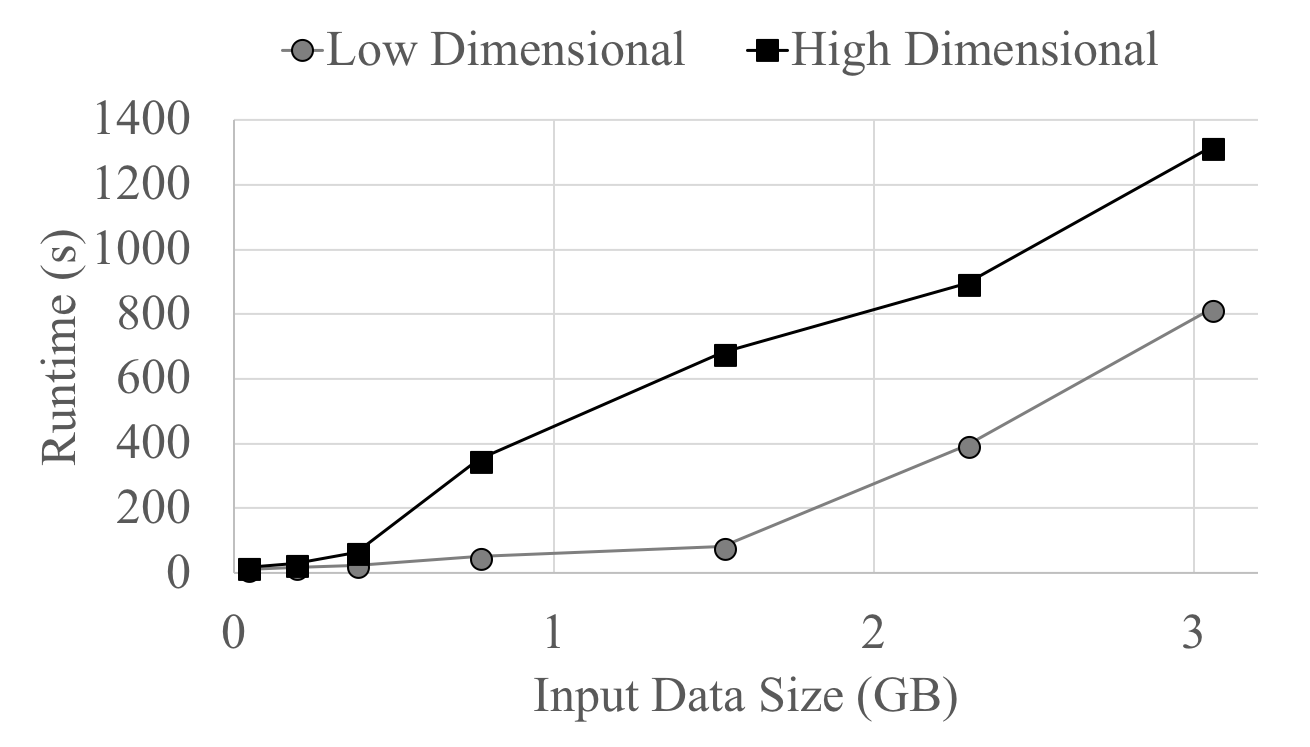
\includegraphics[width=\columnwidth]{figures/spatialjoin.png}
 \caption{We evaluate the execution time of a Ball-Tree join as function of the size of the indexed relation in the high-dimensional and low-dimensional case. As the data structure is increasingly filled the execution time grows non-linearly. \red{What is the scale of the input data on the x axis- KB, MB?}  \label{join} }
\end{figure}

\subsection{Atypical Operator Costs}
In cost-based query optimization, the optimizer uses a cost model to evaluate the cost of different query execution plans. We find that operators in \textsf{DeepLens} pose a few challenges for cost-based optimization. Figure \ref{join} illustrates the difficulties with the execution time of a Ball-Tree join as function of the size of the indexed relation in the high-dimensional and low-dimensional case. As the data structure is increasingly filled the execution time grows non-linearly. The non-linearity is also data-dependent and is more extreme in higher dimensional data. Accurately modeling the relationship between input relation size and operator cost is crucical for cost-based query optimization. The non-linearity of the data structure and the fact that the cost is CPU-bound makes it difficult to analytically model.
The non-linearity also hurts in another way even if we had a perfect analytical model. Join ordering problems are known to be difficult when there are significant non-linearities. Non-linearites can sometimes encourage ``bushy'' joins.

\begin{figure}[t]
% \vspace{-5pt}
\centering
 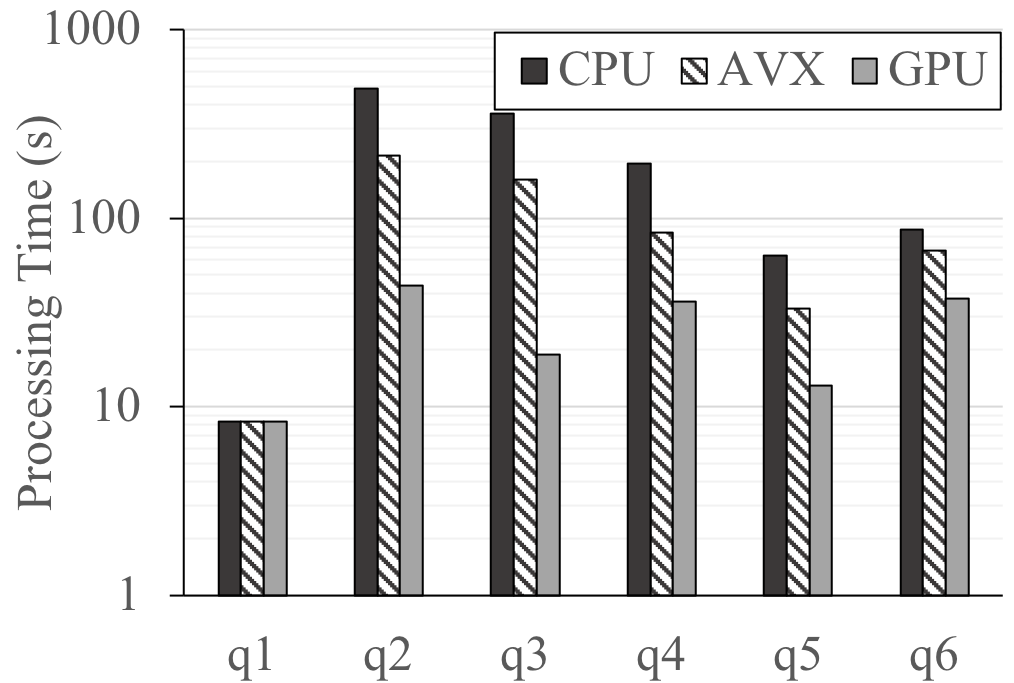
\includegraphics[width=\columnwidth]{figures/build.png}
 \caption{The execution architecture has a considerable impact on the processing time.  \label{build} }
\end{figure}

\subsection{Importance of Architecture}
Compute-bound operations are, by nature, sensitive to the underlying system architecture and execution engine. Figure \ref{build} plots the processing time on each of the six benchmark queries for a vanilla CPU implementation (CPU), a vectorized neural network implementation (AVX), and a GPU implementation (GPU). Just by changing the underlying execution architecture there were up-to 12x changes in execution time. 


